\clearpage
\phantomsection

\setcounter{chapter}{0}
\chapter[{TỔNG QUAN VỀ ĐỀ TÀI}]{TỔNG QUAN VỀ ĐỀ TÀI}

Trước khi tìm hiểu chi tiết về cơ sở lý thuyết hay các thuật toán trong Deep learning hoặc thuật toán YOLO thì ta cần tìm hiểu cơ bản về Deep learning.   

\section{Khái niệm cơ bản}

\subsection{Artificial Neural Network}
Mạng neuron nhân tạo (ANN), là một hệ thống thích nghi được lấy ý tưởng từ não bộ của con người. ANNs là những hệ thống có khả năng thay đổi cấu trúc bên trong của chúng cho một nhiệm vụ nào đó. Ta thường dùng ANN để giải quyết các bài toán phi tuyến tính. \cite{article}

\subsection{Deep learning}
Deep Learning (DL) là một tập con của Machine learning (ML), sử dụng mạng neuron nhân tạo với nhiều lớp (hay còn được gọi là mạng học sâu), lấy ý tưởng từ não bộ của chính con người để mô phỏng khả năng học và đưa ra quyết định một cách nhanh chóng và chính xác của con người. 

Định nghĩa một cách chính xác thì một mạng học sâu, hay deep neural network (DNN), là một mạng neuron nhân tạo với số lớp lớn hơn hoặc bằng 3. Trong các ứng dụng, mạng DNN thường có rất nhiều lớp. Mạng DNN được huấn luyện trên một bộ dữ liệu rất lớn để phân tích và nhận diện các đặc điểm, phân biệt hành vi và mối quan hệ, đánh giá xác suất, đưa ra dự đoán và quyết định. 

Tuy mạng neuron với một lớp có thể đưa ra những dự đoán và quyết định đủ tốt, việc thêm vào nhiều lớp hơn trong mạng neuron đó sẽ giúp tối ưu kết quả với độ chính xác cao hơn.

% \newpage
\section{Convolutional Neural Network}

\subsection{Khái niệm}
Convolutional Neural Network (CNN) hay mạng tích chập, là một loại mạng ANN nhân tạo, cũng được cấu tạo bởi các neuron có khả năng tự tối ưu qua quá trình học. Mỗi neuron sẽ nhận một đầu vào và cho ra đầu ra - chức năng cơ bản của ANN. Điểm khác biệt duy nhất giữa CNN và ANN đó là CNN thường được dùng trong lĩnh vực nhận diện mẫu (pattern) trong ảnh. Điều này cho phép chúng ta mã hóa các đặc điểm đặc biệt của ảnh vào trong kiến trúc mạng, giúp cho mạng CNN trở nên phù hợp hơn cho những công việc liên quan đến ảnh, đồng thời giảm tham số cần thiết cho mô hình. \cite{oshea2015introduction}

\subsection{Vì sao lại là CNN}
Một trong những giới hạn của mạng ANN thông thường chính là việc mạng ANN sẽ có độ phức tạp tính toán rất cao đối với dữ liệu dạng ảnh. Các bộ dữ liệu thông thường được dùng để đánh giá các thuật toán học máy như bộ dữ liệu MNIST, một bộ dữ liệu gồm các chữ số viết tay, sẽ phù hợp cho hầu hết mạng ANN do kích thước của các ảnh là không quá lớn (28 x 28 pixels). Với bộ dữ liệu này, sử dụng mạng ANN thì lớp ẩn đầu tiên sẽ có 784 trọng số (weights) (28 x 28 x 1, 1 ở đây là do bộ dữ liệu MNIST được chuẩn hóa để chỉ có màu đen hoặc trắng), việc này khả thi với hầu hết các loại mạng ANN. Nếu ta xét đầu vào là dữ liệu ảnh màu với kích thước 64 x 64 pixels, số lượng trọng số cho chỉ một neuron của lớp đầu tiên sẽ tăng lên đáng kể. Ta phải tính thêm cả việc để xử lý loại ảnh này, mạng neuron sẽ cần phải lớn hơn rất nhiều so với mạng phân loại ảnh đã được chuẩn hóa của bộ dữ liệu MNIST. \cite{oshea2015introduction}

Trong khi đó, CNN có một điểm khác biệt đó là các neuron trong các lớp của CNN được cấu tạo bởi các neuron được sắp xếp thành 3 chiều, 2 chiều của dữ liệu đầu vào (chiều dài và rộng của ảnh) và chiều sâu. Không giống như ANN thông thường, các neuron trong các lớp của CNN sẽ chỉ kết nối với một phần nhỏ các neuron thuộc lớp trước nó. \cite{oshea2015introduction}

\subsection{Kiến trúc CNN}

\subsubsection{Kiến trúc tổng quan}
CNN gồm 3 lớp cơ bản: lớp tích chập (convolutional layer), lớp tổng hợp (pooling layer), và lớp kết nối đầy đủ (fully-connected layer). 

\subsection{Lớp tích chập}
Lớp tích chập (từ đây sẽ gọi là convolutional layer) là một lớp quan trọng trong kiến trúc mạng CNN, là nơi hầu hết công việc tính toán được thực hiện. Đầu ra của lớp này là các đặc trưng của ảnh dữ liệu đầu vào. 

Ở convolutional layer, ta thực hiện phép tích chập (convolutional) trên ma trận dữ liệu lối vào. Có thể hiểu theo nghĩa lấy một cửa sổ trượt đặt lên từng vùng của ma trận rồi thực hiện phép tích chập. Cửa sổ trượt (sliding window) còn được gọi là kernel, filter hay feature detector.

\begin{figure}[!h]
\center
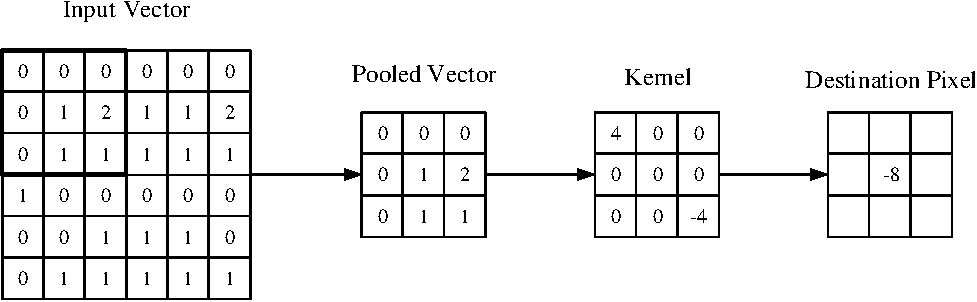
\includegraphics[width=0.8\textwidth]{figures/convlayer.pdf}
\caption{Ví dụ một lớp tích chập\cite{oshea2015introduction}}\label{fig:visual}
\end{figure}
Phần tử ở giữa nhân được đặt trên vector lối vào, sau đó được tính toán và thay bằng tích chập của chính nó với các pixels liền kề nó.

\subsection{Lớp tổng hợp}
Lớp tổng hợp (từ đây sẽ gọi là pooling layer) được sử dụng để giảm số chiều của dữ liệu, qua đó giảm số lượng tham số và độ phức tạp tính toán cho mô hình. 

Pooling layer sẽ được sử dụng trên từng vùng ma trận dữ liệu lối vào, sau đó giảm số chiều của chúng trong khi vẫn giữ lại được những đặc tính quan trọng.  

Pooling layer hoạt động tương tự như convolutional layer, cũng có một cửa sổ trượt gọi là pooling window. Cửa sổ trượt này sẽ trượt qua từng vùng của ma trận lối vào, chọn ra một giá trị từ các giá trị nằm trong vùng cửa sổ trượt. 

Hiện nay có hai loại cửa sổ trượt thường được sử dụng là Max-pooling và Average-pooling. Đối với Max-Pooling, giá trị được chọn ra từ cửa sổ sẽ là giá trị lớn nhất. Còn đối với Average-Pooling thì giá trị được chọn sẽ là giá trị trung bình của các phần tử trong cửa sổ. 

\subsection{Lớp kết nối đầy đủ}
Lớp này tương tự như các lớp thông thường trong mạng ANN, ở đó các neuron sẽ kết nối với mọi neuron thuộc lớp trước của neuron đó. Trước khi đưa ảnh từ lớp trước đó vào lớp này, ta sẽ cần thay đổi chiều của lối vào, cụ thể ta sẽ dàn phẳng dữ liệu lối vào thành một vector cột chứ không còn là dạng ma trận như trước nữa. Tại lớp cuối cùng, ta sử dụng hàm softmax để phân loại đối tượng dựa trên vector đặc trưng đã được tính toán ở các lớp trước đó. 
